% !Mode:: "TeX:UTF-8"

\chapter{}
\textbf{
Show that when all elements are distinct, the best-case running time of HEAPSORT is $\Omega(nlg n)$
}
\hspace*{\fill} \\

%Suppose we have $n$ distinct number $a_1,a_2,...,a_n$.
%In order to simplify our process of prove, we can further suppose that $n=2^k-1$, where $k\in N^{+}$.
%We note $b_1,b_2,...,b_n$ as the heap array order of $a_1,a_2,...,a_n$. According to the process of HEAPSORT, each step of swap the first element and the last element and heapfiying is at
%According to the process of heap construction, the heap is a complete binary tree. Let $k$ be the number of layer. We have
We first prove the lower bound of sorting-based comparison algorithm is $\Omega(nlog n)$.

We can construct a decision-making tree whose node represents a comparison between two elements. Just like the instance showed in figure~\ref{decision_tree},let $k$ be the number of layer of the total decision-making tree. Notice that there are $n!$ kinds of orders and the number of nodes is $2^k$, so we have $2^h\geq n!$.
\begin{figure}[!htbp]
  \centering
  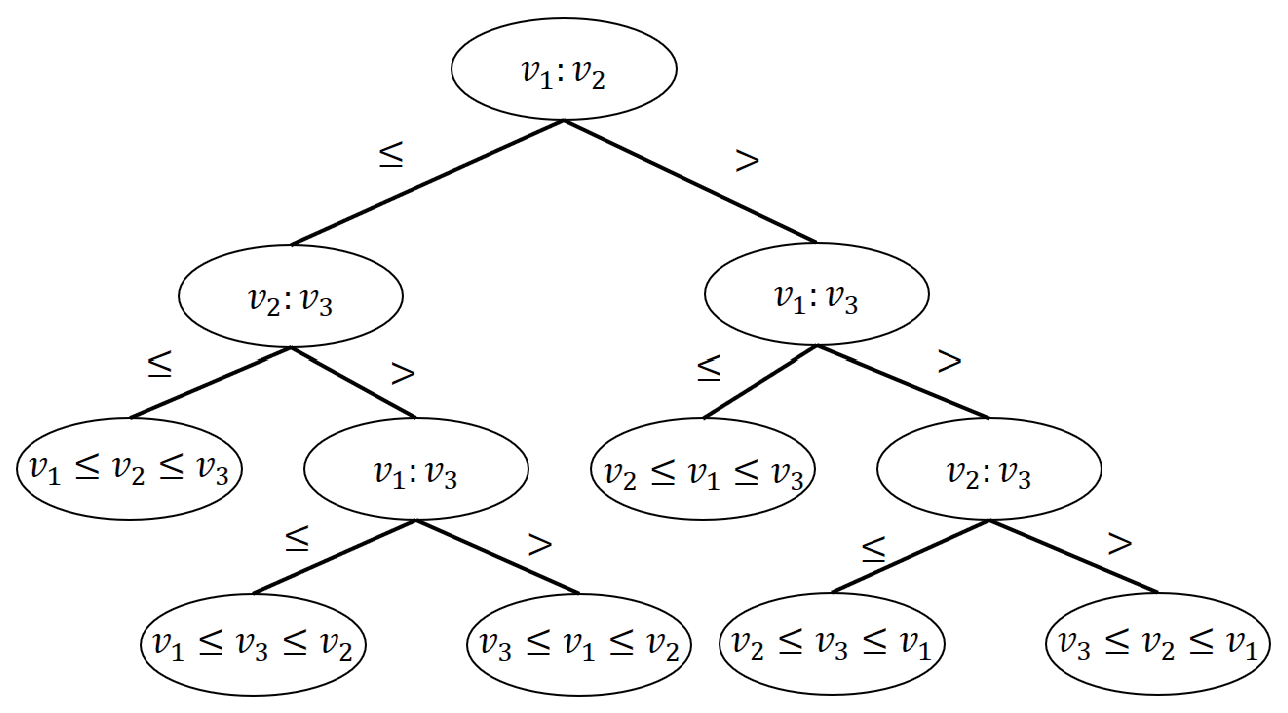
\includegraphics[width=0.7\textwidth]{figures/2_1.eps}\\
  \caption{An instance of decision-making tree}\label{decision_tree}
\end{figure}

Then we can get $h\geq log(n!)$.

According to Stirling's approximation, we have:
$$n!=\sqrt{2\pi n}\cdot (\frac{n}{e})^n\cdot (1+\Theta(\frac{1}{n}))$$

And we can get:
$$h\geq \frac{1}{2}log(2\pi)+\frac{1}{2}log(n)+nlog(n)-nlog(e)+log(1+\Theta(\frac{1}{n}))$$
where
$$\Theta(\frac{1}{n})\in[e^{\frac{1}{12n+1}},e^{\frac{1}{12n}}]$$
So we get the asymptotical lower bound is $\Omega(nlog(n))$.

Because HEAPSORT is one kind of sorting-based comparison algorithm. So we can easily get the best-case running time of HEAPSORT is $\Omega(nlg n)$.
